\section{DFDs}
A data flow diagram (DFD) is a graphical representation of the "flow" of data through an information system, modeling its process aspects. A DFD is often used as a preliminary step to create an overview of the system, which can later be elaborated. DFDs of CMS is as following-:
\begin{enumerate}
\item Data flow LEVEL 0 fig 3.1
\item Data flow LEVEL 1 fig 3.2

\end{enumerate}

A level 0 data flow diagram (DFD), also known as a context diagram, shows a data system as a whole and emphasizes the way it interacts with external entities. This DFD level 0 example shows how such a system might function within a typical retail business.

\begin{figure}[h!]
\centering 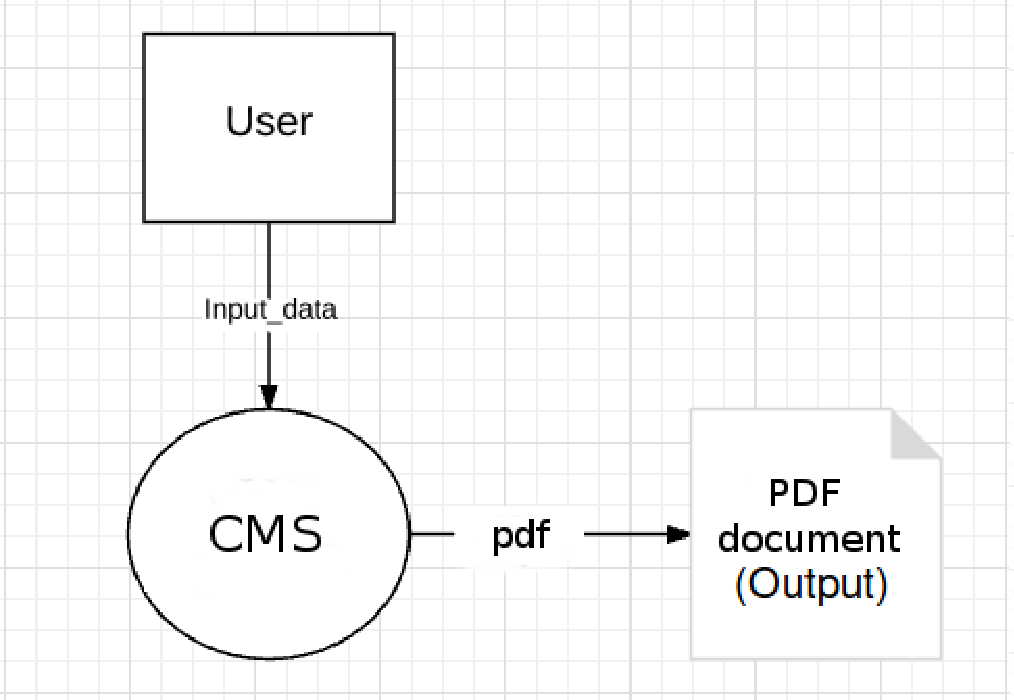
\includegraphics[scale=0.55]{input/images/cms1.pdf}
\caption{Data flow LEVEL 0}
\label{fig:DFDs}
\end{figure}

DFD level 1 breaks down the main processes into subprocesses that can then be analyzed and improved on a more intimate level.\\\\
DFD Level 1 provides a more detailed breakout of pieces of the Context Level Diagram. You will highlight the main functions carried out by the system, as you break down the high-level process of the Context Diagram into its subprocesses.\\\\
Now the Basic Data Flow:-

\begin{figure}[h!]
\centering 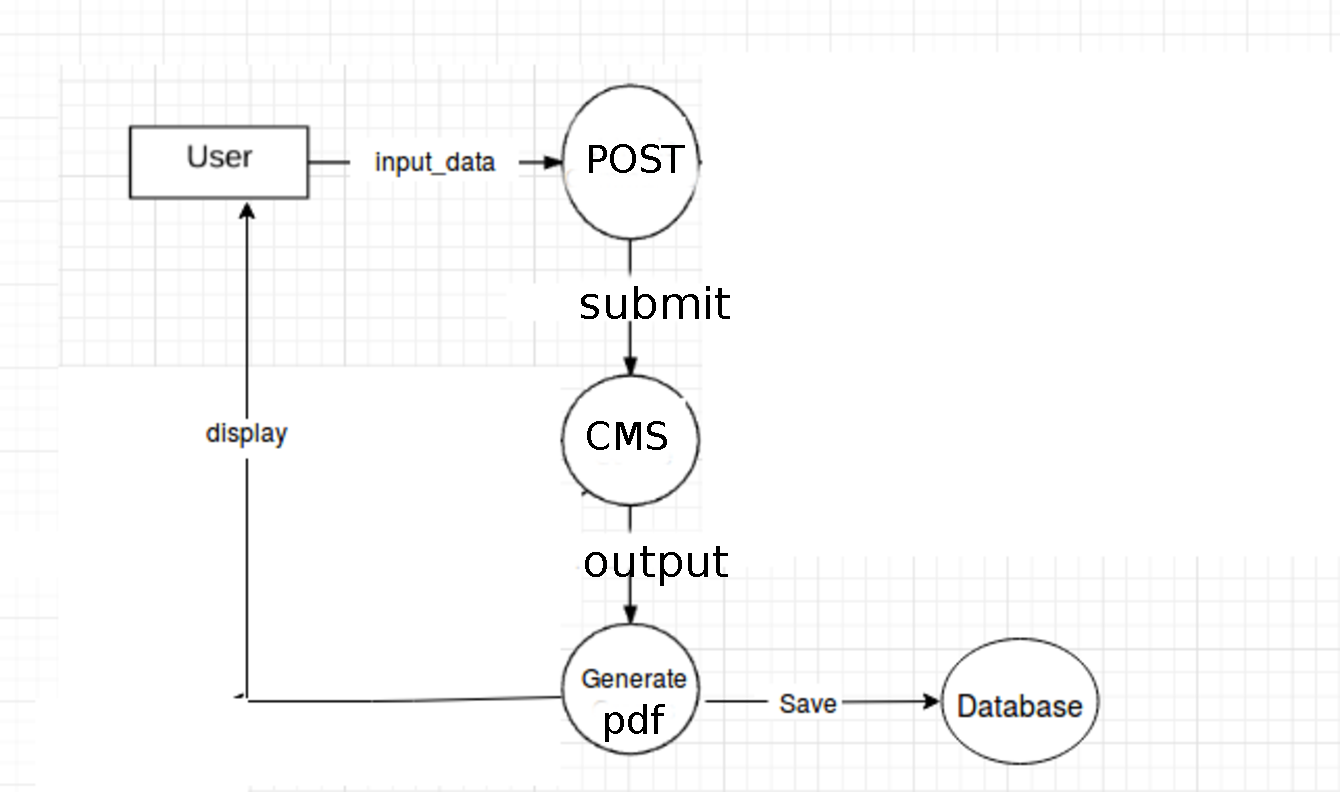
\includegraphics[scale=0.7]{input/images/cms2.pdf}
\caption{Data Flow LEVEL 1}
\label{fig:DFDs}
\end{figure}

\section{Flowchart}
A flowchart is a type of diagram that represents an algorithm, work flow or process, showing the steps as boxes of various kinds, and their order by connecting them with arrows. \\
Flowcharts are used in designing and documenting simple processes or programs. Like other types of diagrams, they help visualize what is going on and thereby help understand a process, and perhaps also find flaws, bottlenecks, and other less-obvious features within it. There are many different types of flowcharts, and each type has its own repertoire of boxes and notational conventions. The two most common types of boxes in a flowchart are:
\begin{enumerate}
\item A processing step, usually called activity, and denoted as a rectangular box.
\item A decision, usually denoted as a diamond.
\item The terminator symbol marks the starting or ending point of the system. It usually contains the word "Start" or "End".
\item A printed document or report is represented by a Document Symbol.
\end{enumerate}
Following is flowchart of system showing flow of control and Data in the software-:
\newpage
\begin{figure}[h!]
\centering 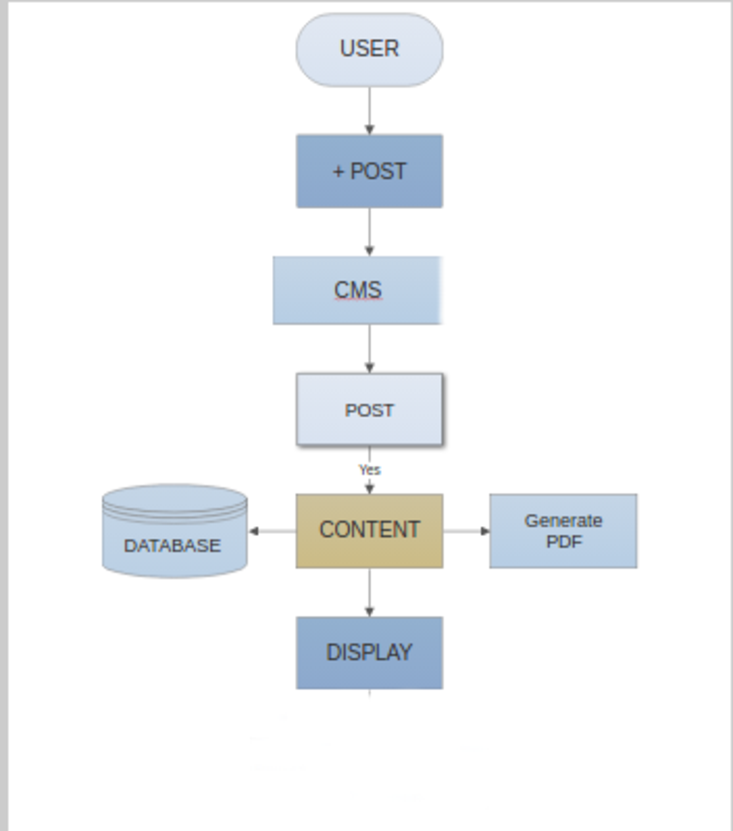
\includegraphics[scale=0.9]{input/images/fc.pdf}
\caption{ Flow diagram}
\label{fig:UI1}
\end{figure}

\section{UI Flow Diagram}
User interface-flow diagrams - also called storyboards, interface-flow diagrams, windows navigation diagrams, and context-navigation maps - enable you to model the high-level relationships between major user interface elements and thereby ask fundamental usability questions. UI Flow diagram tells how user will perceive different interface on click of different buttons or trigger. The rectangular blocks represent entities and Arrow represents change of view from one to another on the bases of button clicked mentioned near arrow. 


